\chapter{Конденсируй-Умножай}
\label{ch:chap3}
Параметры системы:
$$
 C = 277 \mu F
$$
Дано уравнение конденсатора, сразу можно понять тип звена - \textit{идеальное интегрирующее}:
$$
I = C\frac{dU}{dt}
$$


\section{Передаточная функция}
Перейдем в операторную форму Лапласа:
$$
I(s) = CsU(s)
$$
$$
W(s) = \frac{U}{I} = \frac{1}{Cs}
$$
Общий вид идеально-интегрирующего звена:
$$
W(S) = \frac{K}{s}
$$ Тогда в нашем случае $K = \frac{1}{C} \approx 3610$
\section{Временные  характеристики}
$$
y_{i.r.}(t) = \mathcal{L}^{-1}\{\frac{1}{Cs}\} = \frac{1}{C} \approx 3610
$$
$$
y_{s.r.}(t) = \mathcal{L}^{-1}\{\frac{1}{Cs^2}\} = \frac{1}{C}t \approx 3610t
$$

\newpage
\begin{figure}[ht]
  \centering
  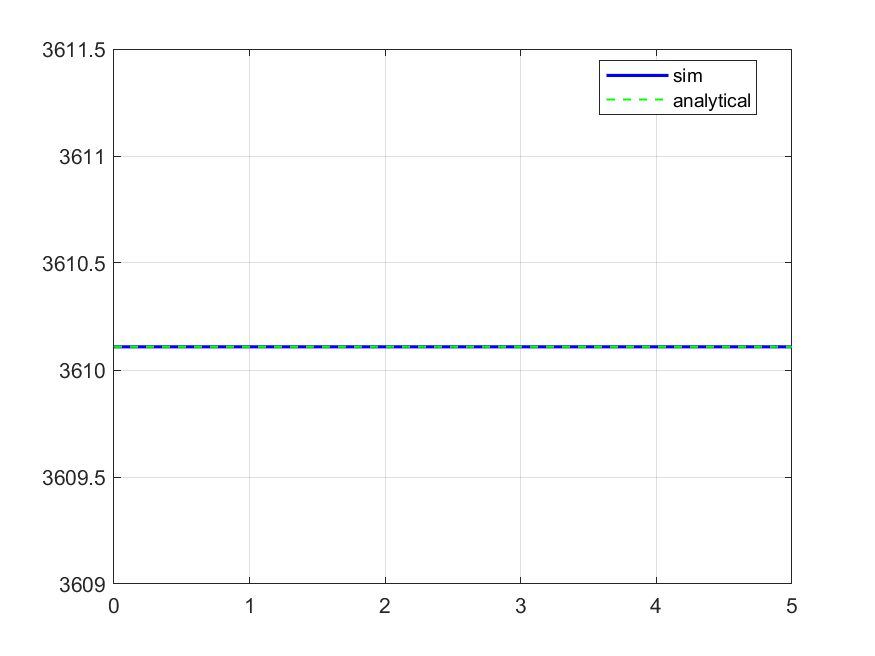
\includegraphics[width=0.8\textwidth]{impulse_responce3.png}
  \caption{Воздействие - \textrm{impulse responce}}
\end{figure}

\begin{figure}[ht]
    \centering
    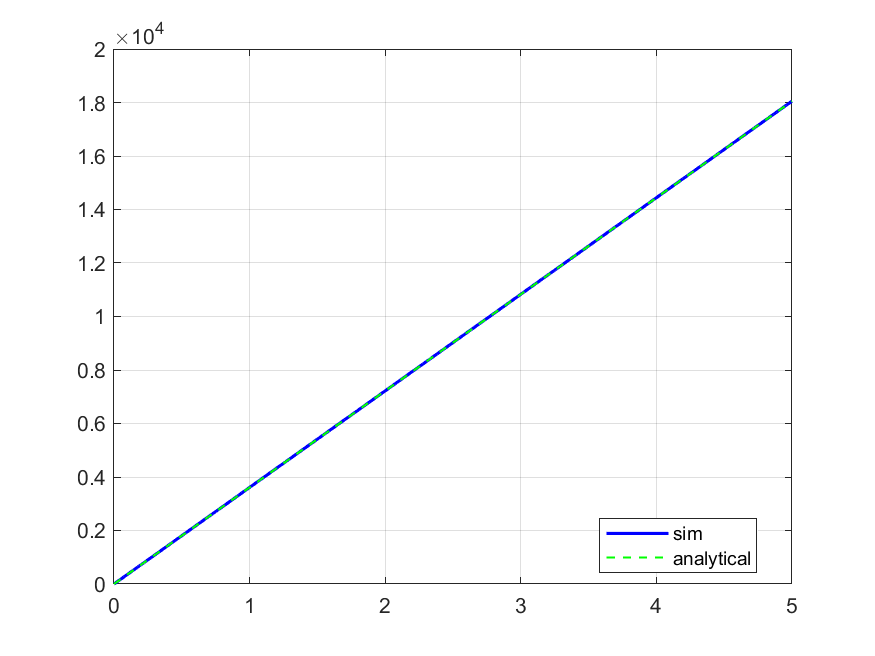
\includegraphics[width=0.8\textwidth]{step_responce3.png}
    \caption{Воздействие - \textrm{step responce}}
  \end{figure}
\newpage

\section{Частотные характеристики}
$$
W(j\omega) =  \frac{1}{Cj\omega} = 0 - j\frac{1}{C\omega}
$$
Амплитудно-частотная характеристика:
$$
A(\omega) = \sqrt{P^2 + Q^2} = \sqrt{0^2 + (\frac{1}{C\omega})^2} = \frac{1}{C\omega} = \frac{3610}{\omega}
$$
Логарифмическая-Амплитудно-частотная характеристика:
$$
L(\omega) = 20lg(A) = 20lg(3610) - 20lg(\omega)
$$
Фазовая-частотная характеристика:
$$
\phi(\omega) = atan2(Q,P) = -\frac{\pi}{2}
$$
\newpage
\begin{figure}[ht]
  \centering
  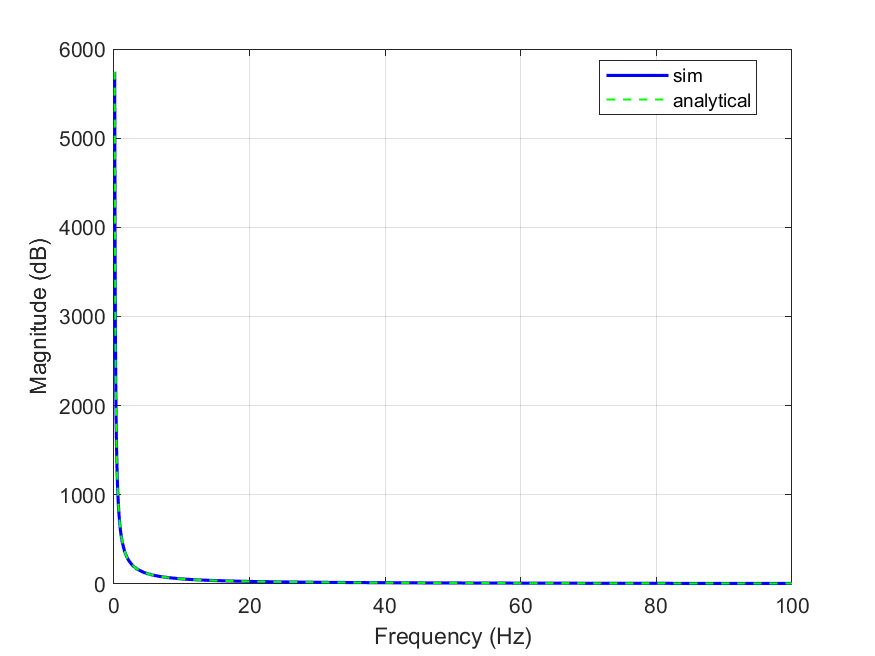
\includegraphics[width=0.8\textwidth]{freq_ampl3.png}
\caption{Сравнение - АЧХ}
\end{figure}

\begin{figure}[ht]
    \centering
    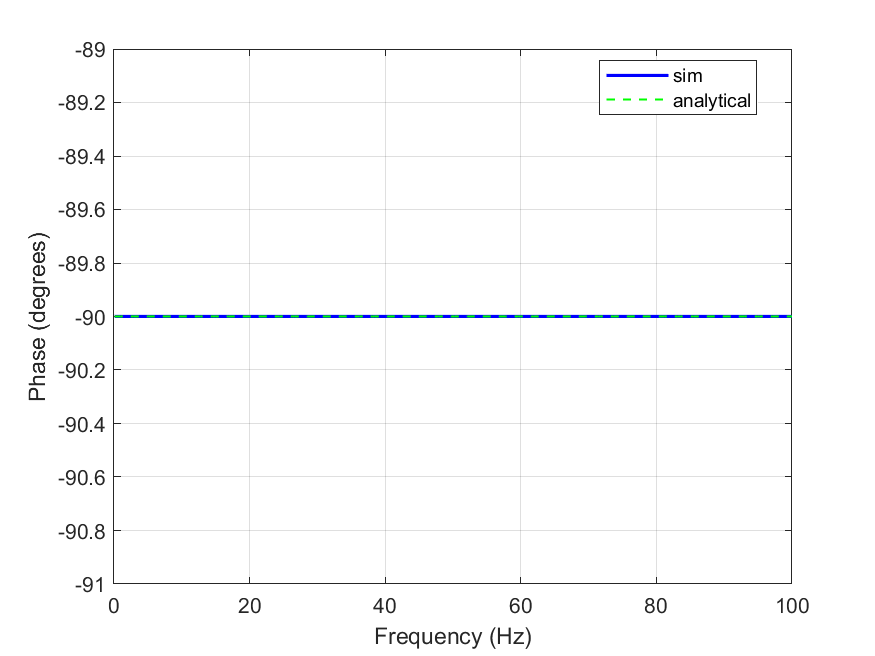
\includegraphics[width=0.8\textwidth]{freq_phase3.png}
  \caption{Сравнение - ФЧХ}
  \end{figure}
\newpage
\begin{figure}[ht]
    \centering
    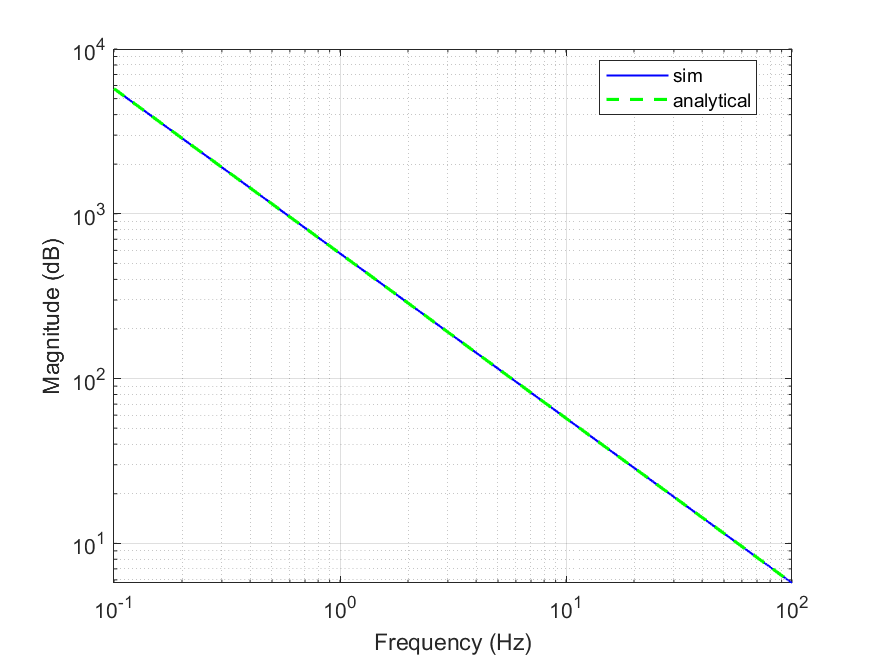
\includegraphics[width=0.8\textwidth]{lfreq_ampl3.png}
  \caption{Сравнение - ЛАЧХ}
  \end{figure}
  
  \begin{figure}[ht]
      \centering
      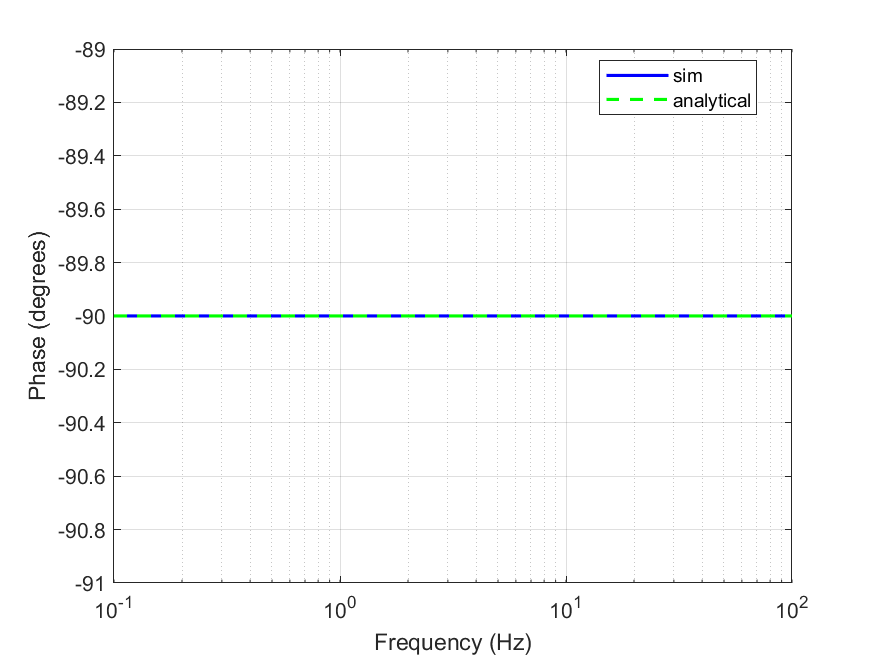
\includegraphics[width=0.8\textwidth]{lfreq_phase3.png}
    \caption{Сравнение - ЛФЧХ}
    \end{figure}
    
    % \begin{figure}[ht]
    %   \centering
    %   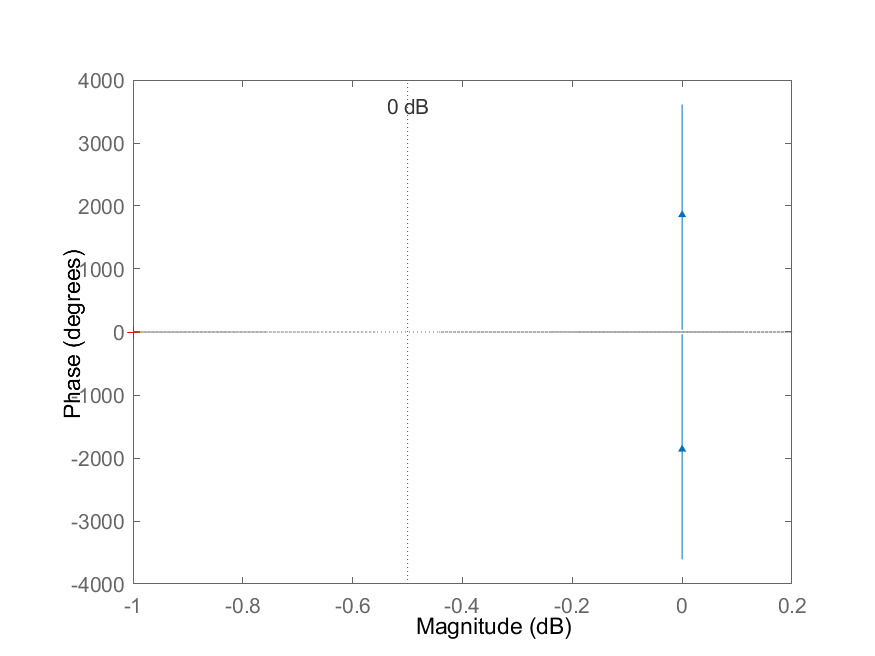
\includegraphics[width=0.8\textwidth]{nyquist3.png}
    % \caption{АФЧХ}
    % \end{figure}
\newpage

\endinput